% Options for packages loaded elsewhere
\PassOptionsToPackage{unicode}{hyperref}
\PassOptionsToPackage{hyphens}{url}
%
\documentclass[
]{book}
\usepackage{amsmath,amssymb}
\usepackage{iftex}
\ifPDFTeX
  \usepackage[T1]{fontenc}
  \usepackage[utf8]{inputenc}
  \usepackage{textcomp} % provide euro and other symbols
\else % if luatex or xetex
  \usepackage{unicode-math} % this also loads fontspec
  \defaultfontfeatures{Scale=MatchLowercase}
  \defaultfontfeatures[\rmfamily]{Ligatures=TeX,Scale=1}
\fi
\usepackage{lmodern}
\ifPDFTeX\else
  % xetex/luatex font selection
\fi
% Use upquote if available, for straight quotes in verbatim environments
\IfFileExists{upquote.sty}{\usepackage{upquote}}{}
\IfFileExists{microtype.sty}{% use microtype if available
  \usepackage[]{microtype}
  \UseMicrotypeSet[protrusion]{basicmath} % disable protrusion for tt fonts
}{}
\makeatletter
\@ifundefined{KOMAClassName}{% if non-KOMA class
  \IfFileExists{parskip.sty}{%
    \usepackage{parskip}
  }{% else
    \setlength{\parindent}{0pt}
    \setlength{\parskip}{6pt plus 2pt minus 1pt}}
}{% if KOMA class
  \KOMAoptions{parskip=half}}
\makeatother
\usepackage{xcolor}
\usepackage{color}
\usepackage{fancyvrb}
\newcommand{\VerbBar}{|}
\newcommand{\VERB}{\Verb[commandchars=\\\{\}]}
\DefineVerbatimEnvironment{Highlighting}{Verbatim}{commandchars=\\\{\}}
% Add ',fontsize=\small' for more characters per line
\usepackage{framed}
\definecolor{shadecolor}{RGB}{248,248,248}
\newenvironment{Shaded}{\begin{snugshade}}{\end{snugshade}}
\newcommand{\AlertTok}[1]{\textcolor[rgb]{0.94,0.16,0.16}{#1}}
\newcommand{\AnnotationTok}[1]{\textcolor[rgb]{0.56,0.35,0.01}{\textbf{\textit{#1}}}}
\newcommand{\AttributeTok}[1]{\textcolor[rgb]{0.13,0.29,0.53}{#1}}
\newcommand{\BaseNTok}[1]{\textcolor[rgb]{0.00,0.00,0.81}{#1}}
\newcommand{\BuiltInTok}[1]{#1}
\newcommand{\CharTok}[1]{\textcolor[rgb]{0.31,0.60,0.02}{#1}}
\newcommand{\CommentTok}[1]{\textcolor[rgb]{0.56,0.35,0.01}{\textit{#1}}}
\newcommand{\CommentVarTok}[1]{\textcolor[rgb]{0.56,0.35,0.01}{\textbf{\textit{#1}}}}
\newcommand{\ConstantTok}[1]{\textcolor[rgb]{0.56,0.35,0.01}{#1}}
\newcommand{\ControlFlowTok}[1]{\textcolor[rgb]{0.13,0.29,0.53}{\textbf{#1}}}
\newcommand{\DataTypeTok}[1]{\textcolor[rgb]{0.13,0.29,0.53}{#1}}
\newcommand{\DecValTok}[1]{\textcolor[rgb]{0.00,0.00,0.81}{#1}}
\newcommand{\DocumentationTok}[1]{\textcolor[rgb]{0.56,0.35,0.01}{\textbf{\textit{#1}}}}
\newcommand{\ErrorTok}[1]{\textcolor[rgb]{0.64,0.00,0.00}{\textbf{#1}}}
\newcommand{\ExtensionTok}[1]{#1}
\newcommand{\FloatTok}[1]{\textcolor[rgb]{0.00,0.00,0.81}{#1}}
\newcommand{\FunctionTok}[1]{\textcolor[rgb]{0.13,0.29,0.53}{\textbf{#1}}}
\newcommand{\ImportTok}[1]{#1}
\newcommand{\InformationTok}[1]{\textcolor[rgb]{0.56,0.35,0.01}{\textbf{\textit{#1}}}}
\newcommand{\KeywordTok}[1]{\textcolor[rgb]{0.13,0.29,0.53}{\textbf{#1}}}
\newcommand{\NormalTok}[1]{#1}
\newcommand{\OperatorTok}[1]{\textcolor[rgb]{0.81,0.36,0.00}{\textbf{#1}}}
\newcommand{\OtherTok}[1]{\textcolor[rgb]{0.56,0.35,0.01}{#1}}
\newcommand{\PreprocessorTok}[1]{\textcolor[rgb]{0.56,0.35,0.01}{\textit{#1}}}
\newcommand{\RegionMarkerTok}[1]{#1}
\newcommand{\SpecialCharTok}[1]{\textcolor[rgb]{0.81,0.36,0.00}{\textbf{#1}}}
\newcommand{\SpecialStringTok}[1]{\textcolor[rgb]{0.31,0.60,0.02}{#1}}
\newcommand{\StringTok}[1]{\textcolor[rgb]{0.31,0.60,0.02}{#1}}
\newcommand{\VariableTok}[1]{\textcolor[rgb]{0.00,0.00,0.00}{#1}}
\newcommand{\VerbatimStringTok}[1]{\textcolor[rgb]{0.31,0.60,0.02}{#1}}
\newcommand{\WarningTok}[1]{\textcolor[rgb]{0.56,0.35,0.01}{\textbf{\textit{#1}}}}
\usepackage{longtable,booktabs,array}
\usepackage{calc} % for calculating minipage widths
% Correct order of tables after \paragraph or \subparagraph
\usepackage{etoolbox}
\makeatletter
\patchcmd\longtable{\par}{\if@noskipsec\mbox{}\fi\par}{}{}
\makeatother
% Allow footnotes in longtable head/foot
\IfFileExists{footnotehyper.sty}{\usepackage{footnotehyper}}{\usepackage{footnote}}
\makesavenoteenv{longtable}
\usepackage{graphicx}
\makeatletter
\def\maxwidth{\ifdim\Gin@nat@width>\linewidth\linewidth\else\Gin@nat@width\fi}
\def\maxheight{\ifdim\Gin@nat@height>\textheight\textheight\else\Gin@nat@height\fi}
\makeatother
% Scale images if necessary, so that they will not overflow the page
% margins by default, and it is still possible to overwrite the defaults
% using explicit options in \includegraphics[width, height, ...]{}
\setkeys{Gin}{width=\maxwidth,height=\maxheight,keepaspectratio}
% Set default figure placement to htbp
\makeatletter
\def\fps@figure{htbp}
\makeatother
\setlength{\emergencystretch}{3em} % prevent overfull lines
\providecommand{\tightlist}{%
  \setlength{\itemsep}{0pt}\setlength{\parskip}{0pt}}
\setcounter{secnumdepth}{5}
\usepackage{booktabs}
\ifLuaTeX
  \usepackage{selnolig}  % disable illegal ligatures
\fi
\usepackage[]{natbib}
\bibliographystyle{apalike}
\IfFileExists{bookmark.sty}{\usepackage{bookmark}}{\usepackage{hyperref}}
\IfFileExists{xurl.sty}{\usepackage{xurl}}{} % add URL line breaks if available
\urlstyle{same}
\hypersetup{
  pdftitle={Machine Learning für das KMU},
  pdfauthor={Martin Sterchi},
  hidelinks,
  pdfcreator={LaTeX via pandoc}}

\title{Machine Learning für das KMU}
\author{Martin Sterchi}
\date{2023-12-22}

\begin{document}
\maketitle

{
\setcounter{tocdepth}{1}
\tableofcontents
}
\hypertarget{uxfcber-das-buch}{%
\chapter*{Über das Buch}\label{uxfcber-das-buch}}
\addcontentsline{toc}{chapter}{Über das Buch}

Die Motivation für dieses Buch kam aus der Erkenntnis, dass viele kleine und mittelgrosse Unternehmen (KMU) in der Schweiz zwar über grosse Datenmengen verfügen, aber nicht das nötige Knowhow haben, um die Daten zu analysieren und für die Optimierung von Entscheidungsprozessen zu nutzen. Mit diesem Buch möchte ich einen kleinen Beitrag leisten, den Knowhow Transfer von Fachhochschulen in die Unternehmen zu katalysieren.

Das Buch versucht, sowohl die klassischen Machine Learning Methoden als auch neueste Entwicklungen im Deep Learning mit einem Fokus auf die Anwendung zu vermitteln. Deep Learning kann als eine Teilmenge des Machine Learnings gesehen werden. Das heisst, jede Deep Learning Methode ist automatisch auch eine Machine Learning Methode. Machine Learning entält jedoch weitere Methoden, welche nicht dem Deep Learning zugeordnet werden können. Das Gebiet Machine Learning ist wiederum eine Teilmenge der Methoden der Künstlichen Intelligenz. Letztere enthält weitere Methoden, welche nicht dem Machine Learning zuzuordnen sind. Abbildung \ref{fig:kimldl} versucht diesen Sachverhalt schematisch darzustellen.

\begin{figure}

{\centering 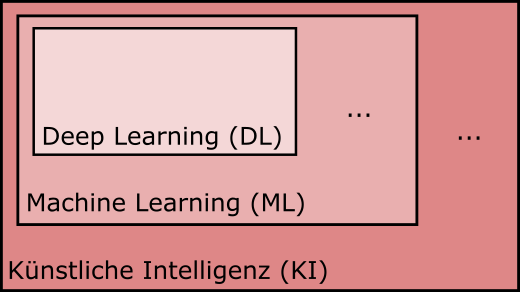
\includegraphics[width=0.6\linewidth]{images/KI_ML_DL} 

}

\caption{Unterscheidung zwischen KI, ML und DL. }\label{fig:kimldl}
\end{figure}

Wir werden im ganzen Buch die folgenden (üblichen) Abkürzungen verwenden:

\begin{itemize}
\tightlist
\item
  Künstliche Intelligenz = KI (oft spricht man auch von AI, was die Abkürzung für den englischen Begriff \emph{Artificial Intelligence} ist).
\item
  Machine Learning = ML
\item
  Deep Learning = DL
\end{itemize}

Obwohl das Buch einen anwendungsorientierten Ansatz verfolgt, soll die mathematisch-statistische Intuition hinter den beschriebenen Modellen und Methoden nicht zu kurz kommen. Diese Intuition ist aus meiner Sicht zwingend, um beurteilen zu können, ob sich ein Modell überhaupt für ein gegebenes Problem eignet. Am Schluss geht es nämlich darum, dass wir mit dem Einsatz von Machine Learning einen Mehrwert für ein Unternehmen oder für die Gesellschaft schaffen können. Das erfordert, dass wir uns eingehend und kritisch mit den Modellen und deren Eignung für ein gegebenes Problem auseinander setzen.

\hypertarget{zielgruppe}{%
\section*{Zielgruppe}\label{zielgruppe}}
\addcontentsline{toc}{section}{Zielgruppe}

Das Buch richtet sich insbesondere an Fachhochschulstudierende in der deutschsprachigen Schweiz mit einem intrinsischen Interesse an quantitativen Methoden im Allgemeinen und Machine Learning im Besonderen. Vorausgesetzt werden Mathematikkenntnisse auf Stufe Mittelschule (Berufs- oder gymnasiale Matur), d.h. Sie sollten vertraut sein mit den Grundlagen bezüglich mathematischer Funktionen, der Integral- und Differentialrechnung sowie den wichtigsten Resultaten aus der Algebra. Ausserdem gehe ich davon aus, dass Sie bereits eine Einführung in das Thema Statistik besucht haben und Konzepte aus der deskriptiven Statistik (Mittelwert, Median, Varianz, Quantile, etc.) sowie aus der Inferenzstatistik (Verteilungen, statistisches Testen, etc.) bekannt sind.

Bevor Sie sich aber nun Sorgen machen: Kapitel \ref{basics} enthält eine Einführung in die wichtigsten Mathematik- und Statistikgrundlagen, die nötig sind für das Verständnis von Machine Learning Modellen.

Da ich mit diesem Buch einen anwendungsorientierten Ansatz verfolge, werden wir auch in das Programmieren einsteigen. Dazu verwenden wir in diesem Buch die Programmiersprache \texttt{R}. Es werden keine Vorkenntnisse vorausgesetzt. Kapitel \ref{intro-R} enthält eine kurze Einführung in die Programmiersprache \texttt{R} und verweist Sie auf weiterführende Ressourcen zum Thema Programmieren. Jedes Modell, das wir uns anschauen werden, ist mit R-Code dokumentiert, so dass Sie lernen, wie die Modelle in der Praxis angewendet werden können.

\hypertarget{aufbau-des-buchs}{%
\section*{Aufbau des Buchs}\label{aufbau-des-buchs}}
\addcontentsline{toc}{section}{Aufbau des Buchs}

Das Buch enthält folgende Kapitel:

\begin{itemize}
\tightlist
\item
  Kapitel \ref{intro}: Einführung in das Thema Machine Learning mit \textbf{Definitionen} sowie Anwendungsbeispielen.
\item
  Kapitel \ref{basics}: Wichtigste \textbf{Mathematik- und Statistikgrundlagen}, die für das Verständnis der Modelle in den späteren Kapitel elementar sind.
\item
  Kapitel \ref{intro-R}: Einführung in das \textbf{Programmieren} mit \texttt{R} sowie Überblick über die wichtigsten \texttt{R}-Packages, die wir verwenden werden.
\item
  Kapitel \ref{lin-reg}: Hier erlernen wir die Grundmodelle, um \textbf{Regressionsprobleme} zu lösen. Es sind lineare Modelle, was bedeutet, dass die funktionale Form der Modelle linear von den Parametern des Modells abhängen. Grafisch bedeutet dies, dass ein solches Modell im einfachsten Fall durch eine Gerade beschrieben werden kann.
\item
  Kapitel \ref{lin-class}: In diesem Kapitel lernen wir die Grundmodelle für das \textbf{Klassifikationsproblem} kennen. Diese Modelle führen typischerweise zu einer linearen Entscheidungsgrenze (engl. \emph{Decision Boundary}) zwischen den verschiedenen Klassen, die wir unterscheiden oder klassifizieren wollen.
\item
  Kapitel \ref{ml-pipeline}: Damit wir ML in der Praxis anwenden können, lernen wir hier die typische \textbf{ML-Pipeline} kennen. Sie werden die Techniken und Methoden kennen lernen, die es braucht, um überhaupt erst an den Punkt zu kommen, um ein ML-Modell rechnen zu können. Oft werden diese Techniken und Methoden unter dem Begriff Preprocessing der Daten zusammengefasst. Doch die Pipeline endet nicht mit dem Rechnen eines ML-Modells. Danach muss ein Modell evaluiert werden und wenn Sie als Analyst*in zufrieden sind, müssen Sie sich Gedanken machen, wie das Deployment des Modells aussehen soll. Das heisst, wie kann Ihr Modell Dritten zur Verfügung gestellt werden? Wir werden uns hier auch kurz mit den wichtigsten Techniken aus dem Unsupervised Learning befassen.
\item
  Kapitel \ref{trees}: Nach den ersten linearen Modellen für das Regressions- und Klassifikationsproblem lernen wir hier ein flexibleres Modell kennen, nämlich den \textbf{Entscheidungsbaum} (engl. \emph{Decision Tree}). Entscheidungsbäume eignen sich sowohl für das Regressions- als auch für das Klassifikationsproblem. Obwohl sie in realen Projekten typischerweise anderen Modellen unterlegen sind, wenn es um die Vorhersagequalität geht, sind sie trotzdem attraktive Modelle, da sie gut visualisierbar sind.
\item
  Kapitel \ref{ensembles}: Aufbauend auf den Entscheidungsbäumen aus dem vorherigen Kapitel können sehr mächtige Modelle erstellt werden, die in der Praxis oft die besten Vorhersagen liefern. Weil es sich dabei üblicherweise um eine clevere Aggregierung der Resultate einer grossen Anzahl individueller Entscheidungsbäume handelt, werden diese Modelle \textbf{Ensembles} genannt. Wie die individuellen Entscheidungsbäume eignen sich Ensembles sowohl für das Regressions- als auch für das Klassifikationsproblem.
\item
  Kapitel \ref{svm}: Ein weiteres mächtiges Modell, das sich sowohl für das Regressions- als auch für das Klassifikationsproblem eignet, sind die \textbf{Support Vector Machines}. Ihre Popularität ist mit dem Aufstieg von Deep Learning etwas verblasst. Es lohnt sich aber immer noch allemal, diese Familie von Modellen kennen zu lernen, insbesondere auch weil sie nicht als Blackbox-Modelle gelten und theoretisch gut fundiert sind.
\item
  Kapitel \ref{ann}: Ab diesem Kapitel steigen wir in das Thema Deep Learning ein. Sie werden die Architektur von einfachen \textbf{Articial Neural Networks} (ANNs) kennen lernen. Ausserdem schauen wir uns in diesem Kapitel den genialen Backpropagation Algorithmus anhand eines einfachen linearen Regressionsproblems an. Dieser Algorithmus ist der Schlüssel für die viel diskutierten Fortschritte im Bereich der künstlichen Intelligenz, weil er das Trainieren von riesigen Modellen überhaupt erst möglich macht.
\item
  Kapitel \ref{cnn}: Hier lernen wir sogenannte \textbf{Convolutional Neural Networks} (CNNs) kennen. Sie sind die Basis für die Fortschritte auf dem Gebiet Computer Vision und erlauben beispielsweise Anwendungen im Bereich automatische Gesichtserkennung in Bildern oder Videos.
\item
  Kapitel \ref{rnn}: Nach ANNs und CNNs lernen wir hier \textbf{Recurrent Neural Networks} (RNNs) kennen. Diese Modelle bilden die Basis für Probleme, in denen die Daten als Sequenzen vorliegen. Das können einache Zeitreihen (z.B. Börsenkurse) sein, aber auch komplexere Sequenzdaten wie beispielsweise geschriebene oder gesprochene Sprache oder Tonaufnahmen.
\item
  Kapitel \ref{gen-AI}: In diesem letzten Kapitel geht es schliesslich um \textbf{Generative KI}. Wir beschäftigen uns hier also mit Modellen, die nicht nur einfach ein Vorhersageprobleme lösen können, sondern auch neue Inhalte (z.B. Texte, Musik, Bilder) generieren können. Abbildung \ref{fig:genAIExML} enthält als Beispiel den Output einer generativen Software, die basierend auf einem Prompt ein Bild erstellt. Nach dem Lesen dieses Kapitels sollten Sie ein grundlegendes Verständnis für die Funktionsweise von Modellen wie Chat-GPT haben.
\end{itemize}

\begin{figure}

{\centering 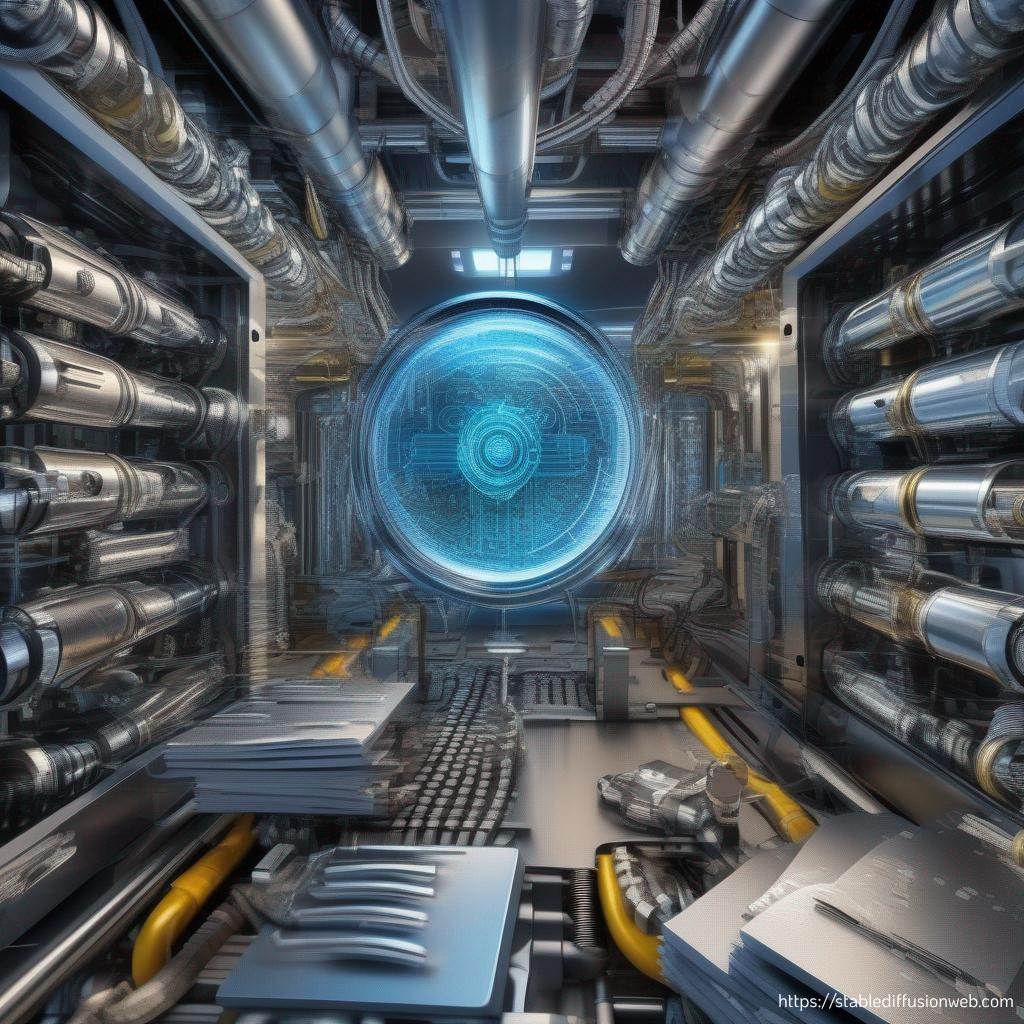
\includegraphics[width=0.7\linewidth]{images/title_picture_ML} 

}

\caption{Beispielsoutput einer generativen Bildgenerierungssoftware (https://stablediffusionweb.com/) basierend auf dem Prompt "A title image for a textbook about Machine Learning targeting small and medium companies."}\label{fig:genAIExML}
\end{figure}

\hypertarget{weiterfuxfchrende-literatur}{%
\section*{Weiterführende Literatur}\label{weiterfuxfchrende-literatur}}
\addcontentsline{toc}{section}{Weiterführende Literatur}

Ein grosser Teil des vorliegenden Buchs baut auf bestehenden Büchern zum Thema Machine Learning auf. Ich werde im Buch immer wieder auf die Quellen verweisen. Die wichtigsten Referenzen für dieses Buch sind folgende:

\begin{itemize}
\tightlist
\item
  Gareth James, Daniela Witten, Trevor Hastie, Robert Tibshirani. (2021). \href{https://www.statlearning.com/}{An Introduction to Statistical Learning: with Applications in R.} New York: Springer. 2nd Edition.
\item
  Aurélien Géron. (2019). \href{https://www.oreilly.com/library/view/hands-on-machine-learning/9781098125967/}{Hands-On Machine Learning with Scikit-Learn, Keras, and TensorFlow: Concepts, Tools, and Techniques to Build Intelligent Systems.} Sebastopol: O'Reilly Media Inc.~3rd Edition.
\item
  Christopher M. Bishop. (2006). \href{https://link.springer.com/book/9780387310732}{Pattern Recognition and Machine Learning.} Berlin, Heidelberg: Springer.
\item
  Kevin P. Murphy. (2012). \href{https://mitpress.mit.edu/9780262018029/machine-learning/}{Machine Learning A Probabilistic Perspective.} The MIT Press.
\end{itemize}

Die ersten beiden Referenzen sind einführende Texte und können parallel zum vorliegenden Buch gelesen werden. Die letzten zwei Referenzen sind fortgeschrittene Texte und ich empfehle, sie erst nach dem vollständigen Verständnis des vorliegenden Buchs oder der ersten beiden Referenzen zu lesen.

\hypertarget{lizenz}{%
\section*{Lizenz}\label{lizenz}}
\addcontentsline{toc}{section}{Lizenz}

Das vorliegende Buch ist unter Lizenz \href{https://creativecommons.org/licenses/by-nc-sa/4.0/deed.de}{CC BY-NC-SA 4.0 DEED} (Namensnennung, nicht-kommerziell, Weitergabe unter gleichen Bedingungen 4.0 International) lizenziert. Bitte halten Sie sich an die Lizenzbedingungen.

\hypertarget{kontakt}{%
\section*{Kontakt}\label{kontakt}}
\addcontentsline{toc}{section}{Kontakt}

Für Fragen und Anregungen zum Buch stehe ich gerne zur Verfügung:

Martin Sterchi\\
Riggenbachstrasse 16\\
4600 Olten\\
\href{mailto:martin.sterchi@fhnw.ch}{\nolinkurl{martin.sterchi@fhnw.ch}}

\hypertarget{intro}{%
\chapter{Einführung}\label{intro}}

In diesem Kapitel geht es darum zu verstehen, was ML überhaupt ist, warum es nützlich sein kann und was typische Anwendungsfälle von ML sind. Wir werden ausserdem verschiedene Unterkategorien von ML kennen lernen.

\hypertarget{was-ist-machine-learning}{%
\section{Was ist Machine Learning?}\label{was-ist-machine-learning}}

Im Prinzip geht die Geschichte des MLs weit zurück, nämlich zu den Anfängen der Statistik. Viele Modelle, die heutzutage im ML angewendet werden sind nämlich eigentlich von Statistiker*innen erfundene Modelle. Die Geschichte des MLs und der Statistik sind darum eng verknüpft. Einen eigentlichen Startpunkt des MLs könnte man vielleicht in den 1960er Jahren ausmachen, mit den Arbeiten von Frank Rosenblatt\footnote{\url{https://en.wikipedia.org/wiki/Frank_Rosenblatt}}, welcher das sogenannte \textbf{Perceptron} und einen dazugehörigen Lernalgorithmus prägte (dazu später mehr). Danach blieb es aber rund 20 Jahre relativ ruhig bis die Forschung im Bereich Machine Learning so richtig Fahrt aufnahm. Ein grosser Schub für die Entwicklung von ML ging vom Aufkommen von extrem grossen Datenmengen (\textbf{Big Data}) und dem Internet aus. Das führte nämlich dazu, dass sich immer mehr Leute aus den Fachbereichen Informatik und Computer Science mit dem Thema ML befassten und effiziente Hard- und Software sowie algorithmische Kniffs und Tricks beisteuerten. Ausserdem ermöglichte das Internet den Zugang zu gewaltigen Datenmengen an Bildern, Videos, Klicks, etc. - denken Sie beispielsweise nur schon an die Informationen, die jede*r von uns tagtäglich im Internet hinterlässt. Ein weiterer Schub für das Machine Learning war (und ist) zudem die immer besser werdende Rechenleistung von Computern. Diese Entwicklungen haben sich im November 2022 kulminiert in der erstmaligen breiten öffentlichen Wahrnehmung von sogenannten \textbf{Large Language Models} wie ChatGPT.

Wie der Name sagt, geht es im ML darum, dass eine Maschine (oder präziser, ein Computer) aus einem gegebenen Datensatz automatisch Muster lernt, ohne dass ein Mensch dem Computer (explizit) sagen muss, was er lernen soll. Der Mensch gibt jedoch dem Computer die Rahmenbedingungen für das selbständige Lernen vor. Die erlernten Muster sind selbstverständlich nur nützlich, wenn sie \textbf{genereller Natur} sind und auch für neue bzw. zukünftige Beobachtungen gelten. Beispiel: ein Spital hat während der Corona Pandemie ein Modell trainiert, um den täglichen Pflegebedarf je nach Wochentag, Saison, und weiteren Indikatoren vorherzusagen. Das Modell funktioniert nun nach der Pandemie aber nicht wunschgemäss und prognostiziert in der Tendenz einen zu hohen Pflegebedarf. Das Problem ist, dass die erlernten Muster nicht gut auf eine Zeit nach der Pandemie generalisierbar sind. Mit anderen Worten: die Trainingsdaten waren nicht repräsentativ genug.

Bevor wir etwas konkreter anschauen, wie genau ein Computer selbständig aus Daten lernen kann, schauen wir uns die Definitionen von zwei Experten im Gebiet ML an:

\emph{``{[}Machine Learning is the{]} field of study that gives computers the ability to learn without being explicitly programmed.''} Arthur Samuel, 1959

\emph{``Machine Learning is the science (and art) of programming computers so they can learn from data.''} Aurélien Géron\footnote{Aurélien Géron. (2019). Hands-On Machine Learning with Scikit-Learn, Keras, and TensorFlow: Concepts, Tools, and Techniques to Build Intelligent Systems. Sebastopol: O'Reilly Media Inc.~3rd Edition.}

Zusammenfassend lässt sich sagen, dass wir mit ML dem Computer die Möglichkeit geben, automatisch und selbständig aus Daten zu lernen. Nichtsdestotrotz braucht es Sie als ML-Expert*in, und zwar wie folgt:

\begin{enumerate}
\def\labelenumi{\arabic{enumi}.}
\tightlist
\item
  Sie entscheiden sich für ein spezifisches ML Modell. Typischerweise kann ein ML Modell durch eine mathematische Funktion (siehe Kapitel \ref{basics}) charakterisiert werden. ML Modelle können unterschiedlich flexibel sein und es liegt im Ermessen von Ihnen, wie flexibel das Modell sein soll. Sie müssen bei der Wahl des Modells die Komplexität des Problems berücksichtigen. Grundsätzliche gilt bei der Wahl des Modells, dass flexiblere Modelle komplexere Sachverhalte abbilden können. Ein zu flexibles Modell kann aber zu Overfitting führen, aber dazu später mehr. Dieser Schritt wird im Fachjargon typischerweise \textbf{Model Selection} (Modelauswahl) genannt.
\item
  Sobald Sie das Modell ausgewählt haben, übergeben Sie dem Computer (etwas vereinfacht gesagt) das Modell, einen Datensatz sowie einen Lernalgorithmus. Nun hat der Computer alle Zutaten, um automatisch zu lernen. Doch was lernt er eigentlich? Der Computer lernt die Parameter Ihres gewählten Modells, so dass das Modell sich optimal an die Daten anpasst. Dieser Schritt wird im Fachjargon \textbf{Model Training} (Trainieren des Modells) genannt.
\item
  Falls Sie mit dem erlernten Modell zufrieden sind, können Sie es nun entweder dazu verwenden Vorhersagen zu machen oder um Zusammenhänge in den Daten zu interpretieren und daraus wertvolle Einsichten gewinnen. Dieser Schritt wird im Fachjargon als \textbf{Model Inference} (Modellinferenz) zusammengefasst. Typischerweise sind Sie in der Realität mit dem ersten erlernten Modell allerdings noch nicht zufrieden und gehen zurück zu Schritt 1 und wählen ein anderes Modell.
\end{enumerate}

Es handelt sich bei dieser Vorgehensweise um eine sehr allgemeine Beschreibung des Machine Learning Prozesses. Wie diese drei Schritte konkret funktionieren, werden Sie in den nachfolgenden Kapiteln dieses Buchs erfahren.

\hypertarget{wann-macht-es-sinn-ml-einzusetzen}{%
\section{Wann macht es Sinn ML einzusetzen?}\label{wann-macht-es-sinn-ml-einzusetzen}}

Ein ML Modell zu trainieren kann viel Zeit und Geld kosten. Zum Beispiel müssen Sie unter Umständen überhaupt erst die Daten sammeln (oder von einem Datendienstleister kaufen), um ein Modell zu trainieren. Oder das Projekt ist so komplex, dass Sie als Analyst*in unzählige Stunden benötigen, um die Daten überhaupt erst in eine Form zu bringen, die es erlaubt ein Modell zu trainieren. Für neuartige DL Modelle oder Generative KI kann das Trainieren bzw. Lernen eines Modells durch den reinen Stromverbrauch bzw. die vom Cloud-Betreiber in Rechnung gestellten Kosten so hoch sein, dass sich Ihr ursprüngliches Vorhaben nicht mehr lohnt. Es ist also ungemein wichtig, dass Sie sich vor Projektbeginn gut überlegen, ob ML für Ihr vorliegendes Problem überhaupt Sinn macht und einen Mehrwert generieren kann.

Folgende Daumenregeln\footnote{siehe auch Seiten 6 - 7 in Aurélien Géron. (2019). Hands-On Machine Learning with Scikit-Learn, Keras, and TensorFlow: Concepts, Tools, and Techniques to Build Intelligent Systems. Sebastopol: O'Reilly Media Inc.~3rd Edition.} können Ihnen dabei helfen, zu entscheiden, ob ML für Ihr Projekt Sinn macht:

\begin{itemize}
\tightlist
\item
  Ihr Problem entspricht einem Standard ML-Problem, das bereits mehrfach gelöst wurde und für das es sogenannte ``off-the-shelf'' Lösungen gibt. Beispiel: Sie wollen das Sentiment (positive vs.~negative Grundhaltung) von Social Media Posts über Ihr Unternehmen automatisch klassifizieren. Dazu gibt es viele vortrainierte Modelle, die teilweise gratis verwendet werden können.
\item
  Der manuelle Arbeitsaufwand ist sehr gross, wenn das Problem durch Menschen gelöst werden soll. Das Problem ist aber ansonsten klar strukturiert und benötigt keinen grossen kognitiven Einsatz eines Menschen. Beispiel: In den Post-Verteilzentren werden die von Hand geschriebenen Postleitzahlen (PLZ) problemlos mittels Computer bzw. ML Modellen erkannt und ``gelesen'' und die Briefe und Pakete entsprechend sortiert.
\item
  Komplexe Probleme, in denen ein Mensch keinen Überblick hat, weil so grosse und komplexe Datenmengen vorhanden sind. Wir Menschen haben grosse Mühe damit, in Rohdaten (reinen Datentabellen) irgendwelche Muster zu erkennen. In diesem Fall können wir entweder versuchen, die Daten zu visualisieren oder mithilfe von ML Zusammenhänge zu lernen, die wir sonst nicht erkennen könnten. Ein illustratives Beispiel ist das Anscombe Quartett\footnote{\url{https://de.wikipedia.org/wiki/Anscombe-Quartett}}, das vier kleine Stichproben mit jeweils elf Datenpunkten enthält. Jeder Datenpunkt wird durch eine \(x\) und eine \(y\) Variable beschrieben. Die vier \(x\)- sowie die vier \(y\)-Variablen haben identische Mittelwerte. Erst eine einfache Visualisierung der vier Stichproben mithilfe eines Streudiagramms zeigt die Muster sowie die Unterschiede zwischen den vier Stichproben deutlich auf.
\end{itemize}

\begin{verbatim}
#>    x1 x2 x3 x4    y1   y2    y3    y4
#> 1  10 10 10  8  8.04 9.14  7.46  6.58
#> 2   8  8  8  8  6.95 8.14  6.77  5.76
#> 3  13 13 13  8  7.58 8.74 12.74  7.71
#> 4   9  9  9  8  8.81 8.77  7.11  8.84
#> 5  11 11 11  8  8.33 9.26  7.81  8.47
#> 6  14 14 14  8  9.96 8.10  8.84  7.04
#> 7   6  6  6  8  7.24 6.13  6.08  5.25
#> 8   4  4  4 19  4.26 3.10  5.39 12.50
#> 9  12 12 12  8 10.84 9.13  8.15  5.56
#> 10  7  7  7  8  4.82 7.26  6.42  7.91
#> 11  5  5  5  8  5.68 4.74  5.73  6.89
\end{verbatim}

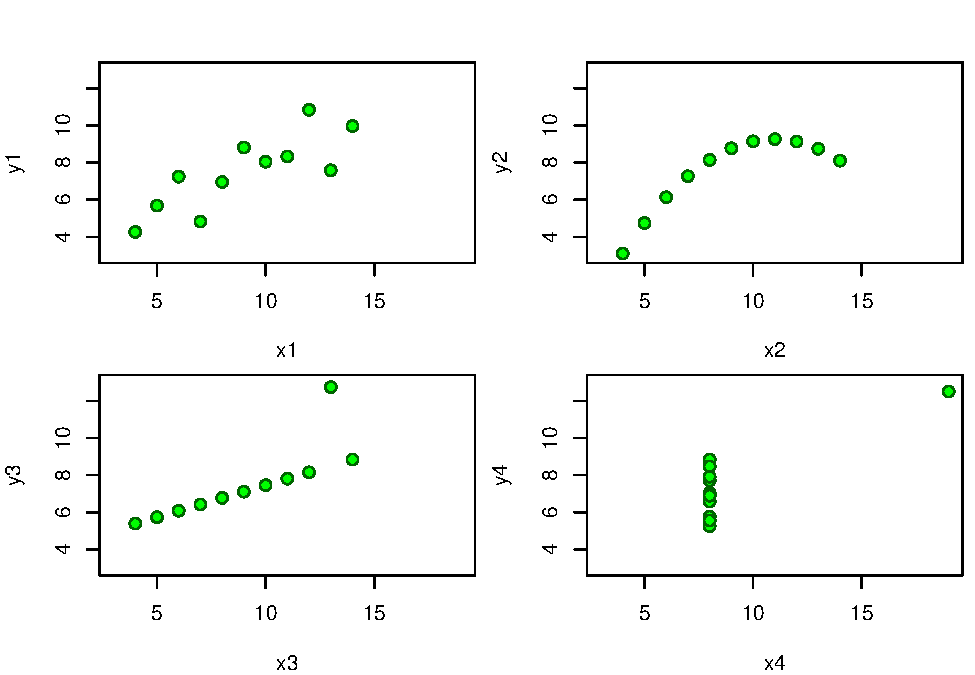
\includegraphics{01-intro_files/figure-latex/anscombe-1.pdf}

\hypertarget{anwendungsfuxe4lle-von-ml}{%
\section{Anwendungsfälle von ML}\label{anwendungsfuxe4lle-von-ml}}

In diesem Abschnitt stelle ich erfolgreiche Anwendungsfälle von ML vor. Einige davon treffen Sie womöglich tagtäglich in Ihrem Alltag an:

\begin{itemize}
\tightlist
\item
  \textbf{Spam Filter} sind ein frühes Beispiel einer erfolgreichen Anwendung von ML. Ein Klassifikationsmodell entscheidet dabei automatisch aufgrund der Inhalte einer Email, des Betreffs sowie des Absenders, ob es sich um eine Spam oder eine sogenannte Ham Email (unproblematische Email) handelt. Falls Sie gängige Email Software verwenden, dann arbeitet im Hintergrund ein Spam Filter daran, Sie vor lästigen Emails zu schützen.
\item
  Ein grosser Teil des wirtschaftlichen Erfolgs von \textbf{Google} basiert auf der Idee, dass aufgrund der Suchhistorie hervorgesagt werden kann, welche Nutzerin oder welcher Nutzer mit welcher Wahrscheinlichkeit eine bestimmte Werbung anklickt. Dies erlaubt Google für jede Nutzer*in die Werbung mit den höchsten ``Erfolgschancen'' zu schalten. Da jeder Klick Einnahmen generiert, ist es für das Geschäftsmodell von Google entscheidend, dass möglichst viele Klicks stattfinden.
\item
  Ein grosser Bereich des MLs und speziell des DLs befasst sich mit \textbf{Computer Vision}. Dabei geht es darum, das Hauptmotiv von Bildern zu klassifizieren (z.B. Zeigt ein Bild ein Tier oder einen Menschen?), Objekte in Bildern zu entdecken (z.B. Enthält das Bild eine Person?) und das entdeckte Objekt dann auch zu klassifizieren (z.B. Handelt es sich bei der Person um XY?). Als konkreteres Beispiel können Sie sich einen Industriebetrieb vorstellen, welcher ein Computer Vision Modell einsetzen möchte, um den Abnützungsgrad der von ihnen produzierten Werkzeuge automatisch zu erkennen und den Kundinnen und Kunden den optimalen Ersatzzeitpunkt für das Werkzeug vorhersagen zu können.
\item
  Ähnlich wie im vorherigen Beispiel gibt es bereits viele Anwendungen im öffentlichen Verkehr, in denen es um \textbf{Predictive Maintenance} geht. Z.B. kann der optimale Wartungszeitpunkt für eine Weiche oder einen Gleisabschnitt aufgrund einer Vielzahl an Indikatoren und Messungen vorhergesagt werden.
\item
  Ein grosses Einsatzgebiet für ML ergibt sich im Finanzsektor durch das automatische Erkennen von potentiell \textbf{betrügerischen Transaktionen}. Falls Sie auch schon mal eine Kreditkartentransaktion direkt am Telefon einer Kundenberaterin oder einem Kundenberater bestätigen mussten, dann ist es wahrscheinlich, dass Ihre Transaktion von einem ML System zur manuellen Überprüfung geflaggt wurde. In diesem Zusammenhang spricht man manchmal auch vom Erkennen von Anomalien (engl. \emph{Anomaly Detection}).
\item
  Sogenannte \textbf{Recommender Systems} sind insbesondere in Online Verkaufspunkten von grossem Nutzen. Betreiben Sie beispielsweise einen grossen Onlinehandel, dann wollen Sie Ihren Kundinnen und Kunden Produkte zum Kauf vorschlagen. Dazu verwenden Sie ein Modell, das basierend auf der Ähnlichkeit zwischen Kundinnen und Kunden potentiell interessante Produkte vorschlägt.
\item
  Die rasanten Entwicklungen im Bereich \textbf{Natural Language Processing} (NLP) in den letzten 10 Jahren haben viele neue und interessante Anwendungsgebiete zutage gefördert. Zum Beispiel eignen sich \emph{Large Language Models} (LLMs) als erste Anlaufstelle für Kundinnen und Kunden (automatisierter Kundenservice). LLMs werden vermutlich aber auch immer mehr in internen Prozessen in Unternehmen eingesetzt, z.B. um komplexe Dokumente zusammenzufassen oder Sitzungsprotokolle zu erstellen.
\end{itemize}

Die obige Liste ist bei weitem nicht komplett und die Entwicklungen im Bereich ML sind aktuell so rasant, dass jeden Tag eine grosse Zahl von neuen ML-basierten Produkten und Dienstleistungen auf den Markt kommen.

\hypertarget{supervised-vs.-unsupervised-learning}{%
\section{Supervised vs.~Unsupervised Learning}\label{supervised-vs.-unsupervised-learning}}

Den Unterschied zwischen dem Supervised Learning und dem Unsupervised Learning können wir am besten erklären, indem wir uns mit ein paar mathematischen Grundlagen des Machine Learnings befassen. Keine Sorge, diese Grundlagen sind sehr einfach, aber versuchen Sie, diese bereits gut zu verstehen, denn wir bauen später darauf auf.

Im \textbf{Supervised Learning} haben wir einerseits sogenannte Input-Daten und andererseits einen Output, den wir vorhersagen wollen. Für die Input-Daten gibt es ganz viele verschiedene Begriffe, die synonym verwendet werden: z.B. Features, unabhängige Variablen, Attribute, Prädiktoren. Dasselbe gilt für den Output, hier gibt es folgende Synonyme: Zielvariable, abhängige Variable, Label, oder auch einfach \(y\). Unsere Konvention hier ist aber folgende: es gibt Input-Daten (oder Input-Variablen) und einen Output (oder Output-Variable).

Die Input-Daten für eine Beobachtung \(i\) schreiben wir mathematisch wie folgt:

\[
\mathbf{x}_i=\begin{pmatrix} x_{i1} \\ x_{i2} \\ \vdots \\ x_{ip} \end{pmatrix},
\]
Diese Notation bedarf ein paar Erklärungen:

\begin{itemize}
\tightlist
\item
  Den Index \(i\) brauchen wir, um die verschiedenen Beobachtungen zu kennzeichnen. \(i\) kann eine Ganzzahl zwischen \(1\) und \(n\) annehmen, wobei \(n\) die Anzahl Beobachtungen im Datensatz bezeichnet. Wenn wir zum Beispiel etwas über die Input-Daten der dritten Beobachtung sagen wollen, dann können wir die Notation \(\mathbf{x}_3\) verwenden.
\item
  Für jede Beobachtung \(i\) haben wir insgesamt \(p\) Variablen, welche die verschiedenen Attribute einer Beobachtung enthalten. \(x_{i1}\) bezeichnet also die erste Variable der i-ten Beobachtung, \(x_{i2}\) die zweite Variable der i-ten Beobachtung und \(x_{ip}\) die p-te (letzte) Variable der i-ten Beobachtung.
\item
  Was Sie oben sehen, ist aus mathematischer Sicht ein Spaltenvektor. Im Moment reicht es, wenn Sie wissen, dass wir mit diesem Spaltenvektor die Input-Daten einer Beobachtung \emph{kompakt} darstellen können.
\end{itemize}

Neben den Input-Daten haben wir im Supervised Learning aber wie erwähnt auch einen Output und den bezeichnen wir üblicherweise mit \(y_i\). Auch hier hilft uns der Index \(i\) dabei, die Beobachtungen eindeutig zu kennzeichnen. Schauen wir uns am besten kurz ein konkretes Beispiel an:

\textbf{Aufgabe}

\textbf{Wichtig}: Beim Supervised Learning geht es um ML Probleme, in denen sowohl Input-Daten als auch ein Output vorhanden ist. Ziel beim Supervised Learning ist es, ein Modell zu trainieren, das basierend auf den Input-Daten möglichst gute Vorhersagen für den Output macht. Es geht also hier um Vorhersageprobleme. In einem gewissen Sinn ist der Output die überwachend Instanz (engl. Supervisor), welche den Lernprozess des Modells kontrolliert.

Im Gegensatz zum Supervised Learning haben wir im \textbf{Unsupervised Learning} nur Input-Daten und \emph{keinen Output}. Im Unsupervised Learning geht es darum, aus den Input-Daten interessante Muster zu lernen, welche für bessere unternehmerische Entscheidungen verwendet werden können. Ein einfaches Beispiel ist das Clustering von Kundinnen und Kunden eines Unternehmens in ähnliche Kundengruppen, so dass die verschiedenen Kundengruppen gezielter mit Marketingaktionen angesprochen werden können. Techniken, um komplexe Datensätze zu visualisieren, werden typischerweise auch zum Unsupervised Learning gezählt.

Neben dem Supervised und dem Unsupervised Learning gibt es noch eine dritte Kategorie von Machine Learning, nämlich das \textbf{Reinforcement Learning} (RL). Dieser Kategorie gehören Modelle an, die (virtuelle) Agenten so trainieren, dass sie langfristig möglichst optimal handeln. Das bekannteste Beispiel aus dem RL ist Googles AlphaGo Agent, welcher den menschlichen Go Weltmeister im Jahr 2017 schlug.\footnote{\url{https://deepmind.google/technologies/alphago/}}. Reinforcement Learning ist aber auch eine wichtige Komponente in der Optimierung von grossen Sprachmodellen wie ChatGPT. In einer ersten Fassung dieses Buchs werden wir uns nicht (oder nur am Rande) mit RL befassen.

Die Unterscheidung zwischen den drei Arten von Machine Learning ist im oberen Teil der Abbildung \ref{fig:slulrl} visualisiert:

\begin{figure}

{\centering 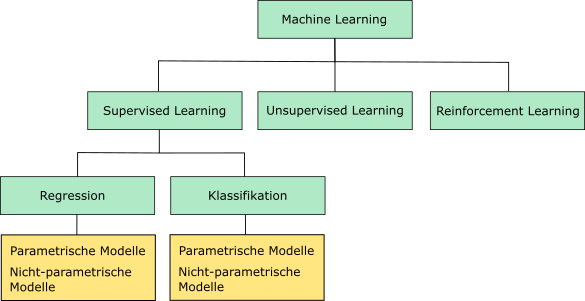
\includegraphics[width=0.9\linewidth]{images/SL_UL_RL} 

}

\caption{Die verschiedenen Kategorien des Machine Learnings und deren Hierarchie. }\label{fig:slulrl}
\end{figure}

\hypertarget{regression-vs.-klassifikation}{%
\section{Regression vs.~Klassifikation}\label{regression-vs.-klassifikation}}

In der Kategorie des Supervised Learnings unterscheiden wir weiter zwischen Regressions- und Klassifikationsproblemen (siehe auch Abbildung \ref{fig:slulrl}).

Im Regressionsproblem ist der Output eine \textbf{stetige} Variable (Intervall- oder Verhältnisskalierung), d.h. die Variable enthält reelle (numerische) Werte. Mathematisch schreibt man dies als \(y_i \in \mathbb{R}\), wobei \(\mathbb{R}\) die Menge der reellen Zahlen beschreibt.

Im Klassifikationsproblem ist der Output bzw. die Zielvariable eine \textbf{kategorische} Variable (Nominal- oder Ordinalskalierung). Mathematisch schreibt man dies als \(y_i \in \{1, \dots, C\}\), wobei \(C\) die Anzahl Kategorien beschreibt. Wenn wir nur \(C=2\) Kategorien haben wie im Beispiel oben mit \(y_i \in \{\text{Betrug}, \text{kein Betrug}\}\) sprechen wir von einem binären Klassifikationsproblem. Falls \(C>2\) sprechen wir vom mehrklassigen (engl. \emph{multiclass}) Klassifikationsproblem.

\textbf{Aufgabe}

\hypertarget{parametrische-vs.-nicht-parametrische-modelle}{%
\section{Parametrische vs.~nicht-parametrische Modelle}\label{parametrische-vs.-nicht-parametrische-modelle}}

Ein ML Modell gehört entweder der Familie \textbf{parametrischer} Modelle oder der Familie \textbf{nicht-parametrischer} Modelle an. Dabei spielt es keine Rolle, ob wir mit dem Modell ein Regressions- oder ein Klassifikationsproblem lösen wollen.

Womöglich sind Sie in Ihrer Ausbildung bereits \textbf{parametrischen Modellen} begegnet, denn das einfache lineare Regressionsmodell ist ein typisches Beispiel für ein parametrisches ML Modell. Das Modell ist vollkommen charakterisiert durch die beiden lernbaren (optimierbaren) Parameter \(w_0\) und \(w_1\)\footnote{In Statistikvorlesungen werden die beiden Parameter oft eher mit \(b_0\) und \(b_1\) oder mit \(\beta_0\) und \(\beta_1\) bezeichnet. Im Machine Learning nennt man Parameter oft Gewichte (engl. Weights), weshalb die Parameter typischerweise mit \(w\) bezeichnet werden.} und kann wie folgt (mathematisch) aufgeschrieben werden:

\[
\hat{y_i} = f(x_i)=w_0 + w_1 \cdot x_i
\]
Wenn Ihnen der obige Ausdruck noch fremd vorkommt, dann ist das nicht schlimm. Wir werden im Kapitel \ref{lin-reg} ausführlich auf lineare Regressionsmodelle eingehen. Im Moment müssen Sie nur wissen, dass ein parametrisches Modell wie oben mit einer mathematischen Funktion beschrieben werden kann und dass diese Funktion durch lernbare \textbf{Parameter} (hier \(w_0\) und \(w_1\)) charakterisiert wird.

\textbf{Nicht-parametrische Modelle} wiederum sind Modelle, welche nicht (oder zumindest nicht explizit) durch Parameter charakterisiert sind. Am besten schauen wir uns gleich ein einfaches nicht-parametrisches Modell an, nämlich das \textbf{K-Nearest-Neighbors} (KNN) Modell. Stellen Sie sich vor, Sie haben einen Datensatz mit 55 Produkten aus Ihrem Sortiment. Sie haben jedes dieser 55 Produkte auf Instagram und auf Tiktok durch Influencer*innen bewerben lassen. Für jedes der 55 Produkte hatten Sie ein Werbebudget für Instagram (\(x_{i1}\)) und ein Werbebudget für Tiktok (\(x_{i2}\)). Am Ende des Geschäftsjahrs haben Sie für jedes der 55 Produkte bestimmt, ob die Absatzziele erreicht wurden oder nicht (Output \(y_i\)). Die erfolgreichen Produkte (= Absatzziel erreicht) sind in untenstehender App als blaue Punkte eingezeichnet. Die roten Dreiecke repräsentieren die nicht-erfolgreichen Produkte. Sie sehen, dass erfolgreiche Produkte tendenziell höhere Instagram und Tiktok Werbebudgets aufwiesen als nicht-erfolgreiche Produkte. Sie möchten nun ein Modell schätzen, dass die Produkte automatisch klassifizieren kann. Dazu verwenden Sie das KNN Modell, das die \(K\) nächsten Nachbarn unter den 55 gegebenen Produkten sucht und dann die häufigste Beobachtung unter den \(K\) nächsten Nachbarn vorhersagt. In anderen Worten: wir suchen die \(K\) \textbf{ähnlichsten} Beobachtungen und nutzen diese, um eine Vorhersage zu machen.

Selbstverständlich spielt der konkrete Wert von \(K\) hier eine grosse Rolle - sollen wir nur \(K=1\) Nachbarn berücksichtigen? Oder \(K=10\) Nachbarn? Die erste Abbildung in der App zeigt nicht nur die 55 Datenpunkte, sondern auch die \textbf{Entscheidungsgrenze} (in schwarz). Untersuchen Sie kurz, wie sich diese Entscheidungsgrenze verändert, wenn Sie \(K\) erhöhen oder reduzieren.

Ausserdem können Sie in der ersten Abbildung auch den schwarzen Punkt mit der Maus setzen, wodurch Ihnen die \(K\) nächsten Punkte des schwarzen Punkts angezeigt werden.

Die zweite Abbildung zeigt die Entscheidungsregionen mit unterschiedlicher Intensität je nachdem wie sicher sich das Modell ist. In einer Region, in der alle \(K\) Nachbarn nicht-erfolgreiche Produkte sind, sind wir uns eher sicher bezüglich der Vorhersage als in einer Region, in der die Anteile zwischen erfolgreichen und nicht-erfolgreichen Produkten ausgeglichen sind.

Um die \(K\) nächsten Nachbarn zu finden, müssen wir die Distanzen zwischen Punkten rechnen können. Dazu verwenden wir die Euklidische Distanz, welche wir in Kapitel \ref{basics} kennen lernen werden.

Das KNN Modell ist ein sehr einfaches ML Modell, welches in der Praxis allerdings nicht allzu häufig angewendet wird. Warum nicht? Weil es am sogenannten \textbf{Fluch der Dimensionalität} (engl. Curse of Dimensionality) leidet. Doch was bedeutet das? Je mehr Input-Variablen wir haben, desto weiter entfernt sind Datenpunkte voneinander (das ist etwas, das man sich nur schwer vorstellen kann, aber Sie können es mir für den Moment einfach mal glauben). Das KNN beruht auf der Grundidee, dass wir \(K\) nahe, ähnliche Beobachtungen für die Vorhersage verwenden. Wenn diese \(K\) nahen Beobachtungen im hochdimensionalen Raum (= viele Input-Variablen) nicht mehr nahe sind, dann funktioniert auch das Modell nicht mehr gut.

\textbf{Aufgaben}

\hypertarget{machine-learning-pipeline}{%
\section{Machine Learning Pipeline}\label{machine-learning-pipeline}}

Abbildung \ref{fig:pipeline} zeigt, wie eine typische ML-Pipeline aussieht.\footnote{Icons stammen von \url{https://thenounproject.com/}.}

\begin{figure}

{\centering 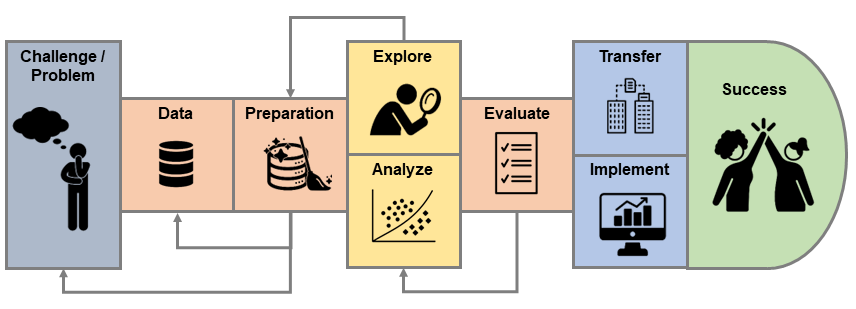
\includegraphics[width=0.9\linewidth]{images/Pipeline} 

}

\caption{Eine typische ML-Pipeline. }\label{fig:pipeline}
\end{figure}

Sie starten typischerweise mit einem \textbf{Problem} oder einer Herausforderung. Ihr ganzes Projekt sollte darauf ausgelegt sein, dieses Problem zu lösen. Es ist grundsätzlich nicht ratsam, auf Biegen und Brechen eine ML Lösung zu implementieren, wenn kein klar definiertes Problem vorliegt. Nehmen Sie sich also zu Beginn eines Projekts Zeit, das Problem grundlegend zu definieren. Sprechen Sie auch mit den entsprechenden Fachexpert*innen im Unternehmen, um genau zu verstehen, was verbessert oder effizienter gemacht werden soll und was die technischen oder ökonomischen Einschränkungen sind.

Sobald das Problemverständnis vorhanden ist, beginnen Sie, sich mit den \textbf{verfügbaren Daten} zu befassen. Auch hier müssen Sie sich wahrscheinlich mit den entsprechenden Expert*innen im Unternehmen (z.B. Datenbankadministrator*innen) austauschen. Es geht hier unter anderem darum abzuklären, welche Daten verfügbar sind, in welchem Format die Daten vorhanden sind wie die Datenqualität ist.

Danach beginnen Sie mit den Datenarbeiten. Häufig wird dieser Schritt \textbf{Preprocessing} oder \textbf{Data Cleaning} genannt. Oft verschlingt dieser Arbeitsschritt sehr viel Zeit und es ist nicht unüblich, dass 80\% der Projektzeit hier aufgewendet werden. Es ist auch völlig normal, wenn Sie von diesem Schritt zurück zur Problemdefinition gehen und sie verfeinern oder anpassen müssen oder zum Beispiel nochmals Fragen mit den Datenbankexpert*innen klären müssen, weil Ihr Datenverständnis noch nicht vollständig ist.

Nachdem die Daten vorbereitet wurden, gehen Sie typischerweise zu einer \textbf{explorativen Analyse} der Daten über. Das heisst, Sie visualisieren die vorhandenen Variablen univariat (d.h. jede Variable einzeln) oder multivariat (d.h. zwei oder mehr Variablen zusammen). Ein Beispiel einer univariaten Visualisierung ist ein Histogramm einer quantitativen Variable (z.B. Quartalsumsätze). Ein Beispiel einer multivariaten Visualisierung ist ein Streudiagramm zweier quantitativer Variablen (z.B. Quartalsumsätze und Wechselkurse). Auch hier ist es üblich, dass Sie einen Schritt zurück gehen und weitere Datenbereinigungen vornehmen müssen.

Nach der explorativen Analyse der Daten sollten Sie eine erste Idee von den wichtigsten Zusammenhängen in den Daten haben. Basierend darauf können Sie Ihr erstes Modell wählen und trainieren und mit der eigentlichen \textbf{Analyse} bzw. der Lösung des Problems beginnen.

Einer der wichtigsten Schritte ist die saubere und gründliche \textbf{Evaluation} Ihrer Modelle. Dieser Schritt dient einerseits dazu das beste Modell auszuwählen und andererseits dazu die Qualität Ihrer Lösung bzw. Ihres Modells abzuschätzen. Mit diesem zweiten Schritt wollen Sie nämlich bereits während der Projektphase einschätzen können, wie gut Ihr Modell das gegebene Problem löst oder einen bestehenden Betriebsprozess verbessert oder effizienter macht. Die beiden Schritte Analyse und Evaluation werden typischerweise ein paar Mal iteriert, bis Sie das beste Modell gefunden haben.

Am Schluss geht es darum, dass Sie Ihr Wissen und Ihre Erkenntnisse an die relevanten Fachexpert*innen weitergeben (\textbf{Wissenstransfer}) und Ihr finales Modell in einer produktiven Umgebung implementieren (oft \textbf{Deployment} genannt). Zum Beispiel können Sie Ihr Modell in einer mobilen App einbetten oder als REST API Service zur Verfügung stellen.

\hypertarget{basics}{%
\chapter{Mathematik- und Statistik-Grundlagen}\label{basics}}

In diesem Kapitel repetieren wir die wichtigsten Grundlagen aus der Mathematik und Statistik, die es braucht, um Machine Learning Modelle zu verstehen. Das Thema \emph{Lineare Algebra} wird für die meisten von Ihnen wahrscheinlich Neuland sein.

\hypertarget{funktionen}{%
\section{Funktionen}\label{funktionen}}

Eine Funktion, die wir in der Mathematik typischerweise mit \(f\) bezeichnen, ordnet jedem \textbf{Argument} \(x\) aus dem Definitionsbereich \(D\) (engl. \emph{Domain}) \textbf{genau einen Wert \(y\)} aus dem Wertebereich \(W\) (engl. \emph{Codomain}) zu. Oft sind \(D\) und \(W\) die Menge der reellen Zahlen, also \(\mathbb{R}\). Die Menge der reellen Zahlen enthält alle möglichen Zahlen, die Sie sich vorstellen können.\footnote{Einzige Ausnahme sind die komplexen Zahlen.} Zum Beispiel die Zahlen \(3\), \(-4.247\), \(\sqrt{14}\), \(5/8\), etc.

Wie eine Funktion grafisch aussieht, ist aus Panel (a) der Abbildung \ref{fig:functions} ersichtlich. Hier zeigen wir die Form einer Funktion in einem kartesischen Koordinatensystem. Die Funktionskurve weist jedem Wert \(x\) auf der x-Achse genau einen Wert \(y\) auf der y-Achse zu. Der wichtigste Teil der oben aufgeführten Definition ist der Teil ``genau einen Wert'', denn eine Funktion kann einem Element \(x\) nicht zwei oder mehr Werte zuweisen, sondern nur genau einen. Genau aus diesem Grund handelt es sich bei Panel (b) in Abbildung \ref{fig:functions} \emph{nicht} um eine Funktion, da gewissen \(x\)-Werten mehrere Werte \(y\) zugeordnet werden. \emph{Wichtig}: das heisst aber nicht, dass zwei verschiedenen \(x\)-Werten, nennen wir sie \(x'\) und \(x''\), derselbe \(y\)-Wert zugeordnet werden kann (vgl. Panel (a)).

\begin{figure}

{\centering 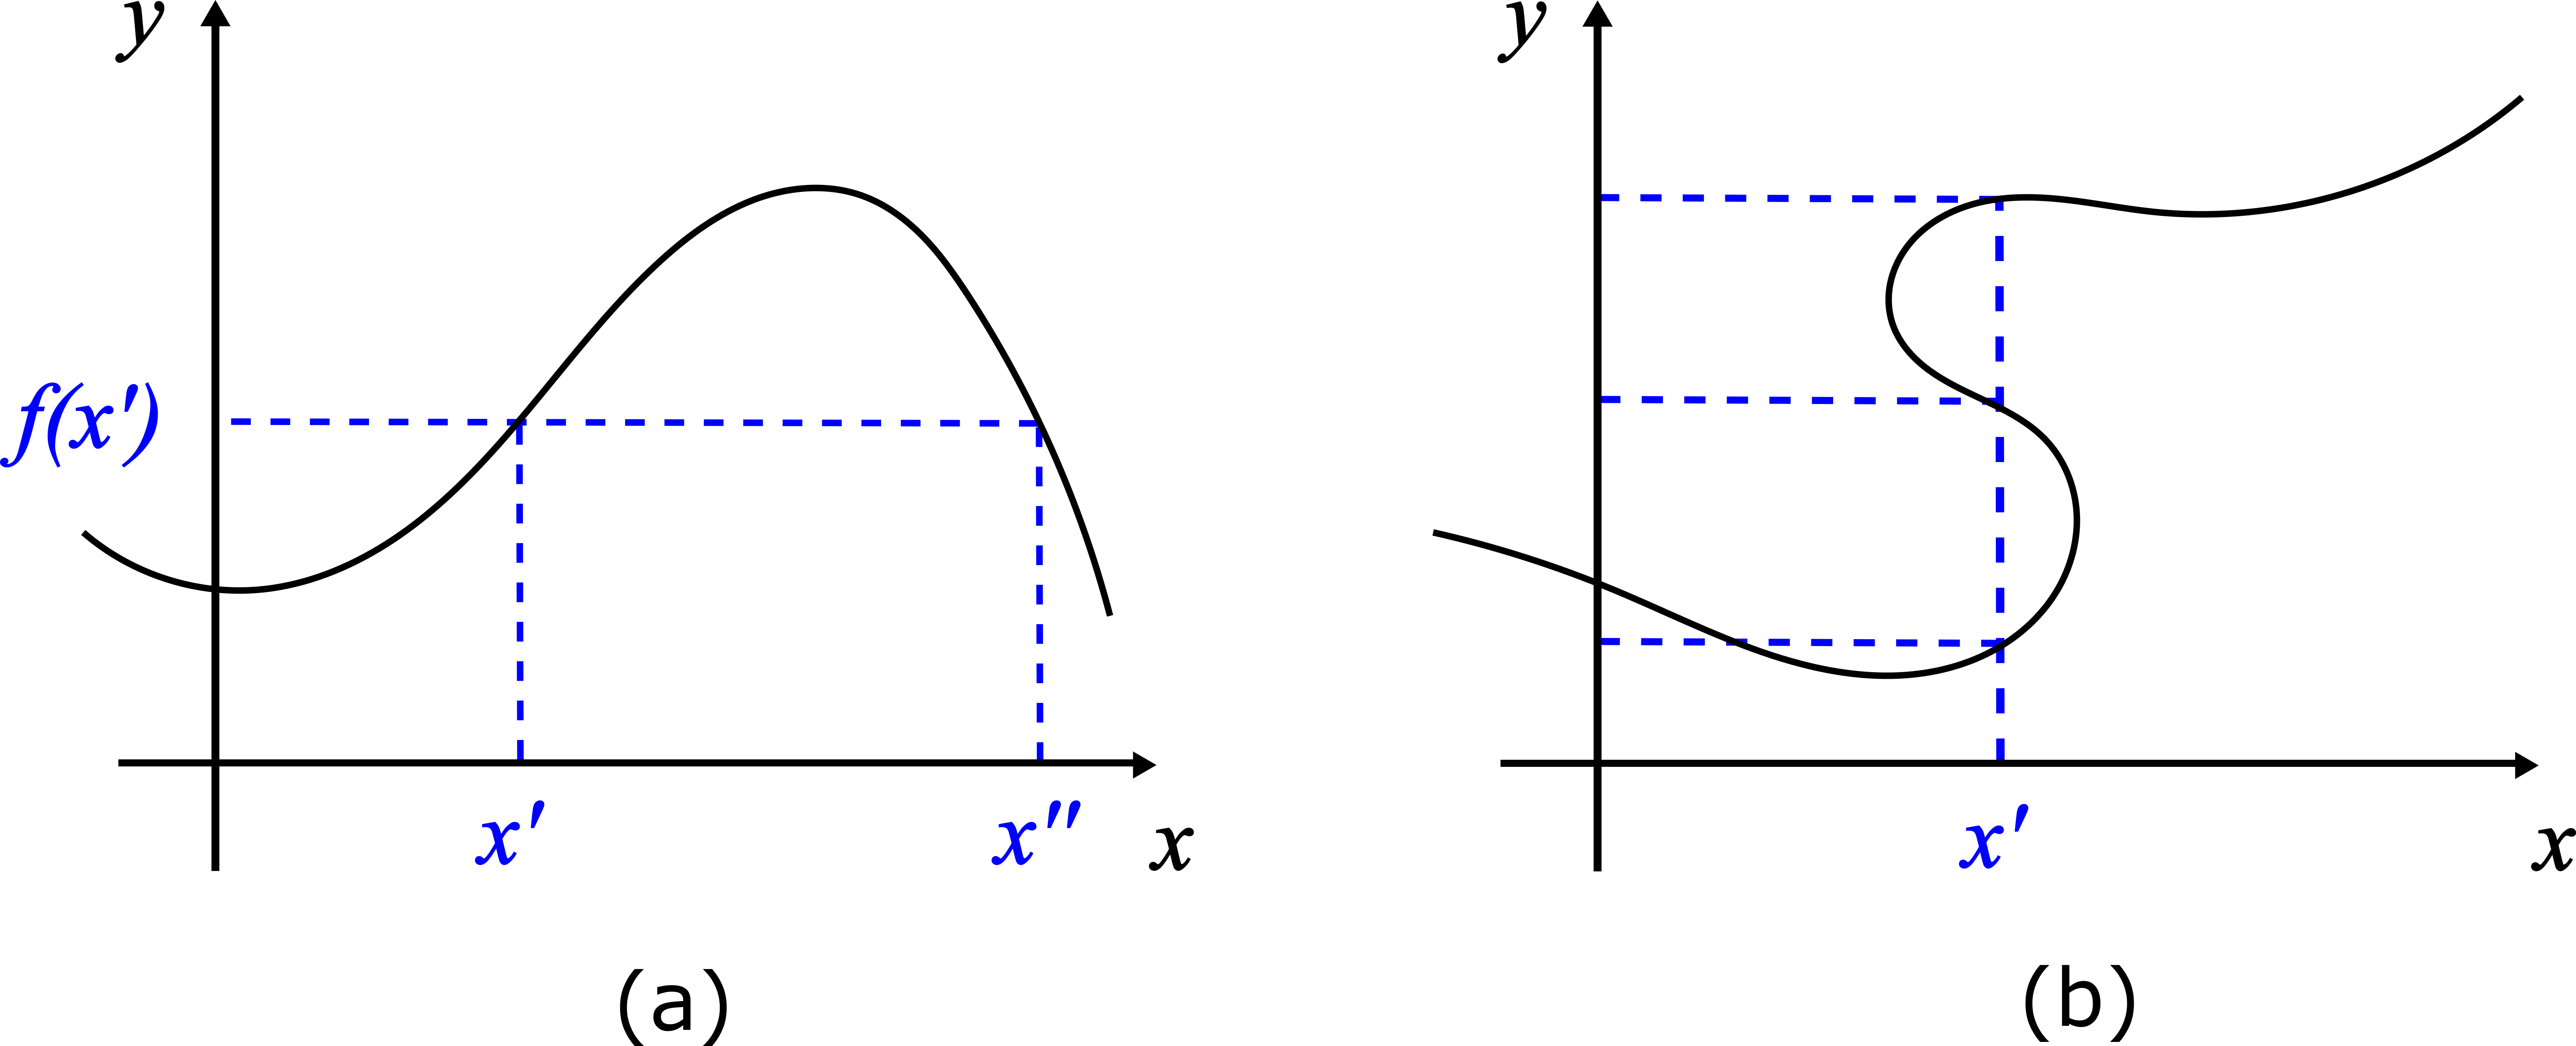
\includegraphics[width=0.8\linewidth]{images/Functions} 

}

\caption{(a) Eine Funktion, die jedem x-Wert genau einen y-Wert zuweist. (b) Keine Funktion. }\label{fig:functions}
\end{figure}

Mathematisch wird diese allgemeine Definition einer Funktion häufig wie folgt beschrieben:

\[
f : x \mapsto y
\]
Wir haben also eine Funktion \(f\), die jedem Element \(x\) genau einen Wert \(y\) zuweist. Der Pfeil in obiger mathematischer Schreibweise beschreibt genau dieses Mapping. Wie genau dieses Mapping einem Argument \(x\) den entsprechenden \(y\)-Wert zuordnet, wird durch die Funktion \(f(x)\) beschrieben. In den folgenden Abschnitten schauen wir uns typische Beispiele von Funktionen an, angefangen mit linearen Funktionen. Doch vorher wollen wir uns kurz überlegen, warum Funktionen für das Machine Learning überhaupt wichtig sind. Ein grosser Teil des Machine Learnings, der \textbf{Supervised Learning} genannt wird, befasst sich mit dem Problem, wie eine Zielvariable \(y\) mithilfe von einem oder mehreren Prädiktoren \(x\) vorhergesagt werden kann. Ein Machine Learning Modell ist darum nichts anderes als eine Funktion \(y=f(x)\), die basierend auf den Prädiktoren \(x\) die Zielvariable \(y\) möglichst gut beschreiben kann.\footnote{Zumindest aus einer nicht-probabilistischen Perspektive.}

\hypertarget{lineare-funktionen}{%
\subsection{Lineare Funktionen}\label{lineare-funktionen}}

Nun schauen wir uns an, wie eine \textbf{lineare} Funktion aussieht. Eine lineare Funktion kann allgemein wie folgt geschrieben werden:

\[
y = f(x) = a \cdot x + b
\]
Obige Funktionsgleichung besagt, dass wir den entsprechenden \(y\)-Wert kriegen, indem wir den Wert des Arguments \(x\) mit \(a\) multiplizieren und danach eine Konstante \(b\) addieren. \(a\) und \(b\) sind die \textbf{Parameter} dieser Funktion. Die konkreten Zahlenwerte dieser beiden Parameter definieren, wie die Funktion am Schluss genau aussieht.

Eine lineare Funktion hat auch eine geometrische Interpretation und zwar entspricht eine lineare Funktion einer Gerade. Das ist auch der Grund, warum wir diese Funktionen \textbf{linear} nennen, sie können graphisch durch eine ``Linie'' dargestellt werden. Der Parameter \(a\) ist die Steigung dieser Geraden und der Parameter \(b\) entspricht dem Ort, wo die Gerade die y-Achse schneidet (sogenannter y-Achsenabschnitt).

Am besten schauen wir uns ein paar konkrete Beispiele an (Abb. \ref{fig:lin-func}).

\begin{figure}

{\centering 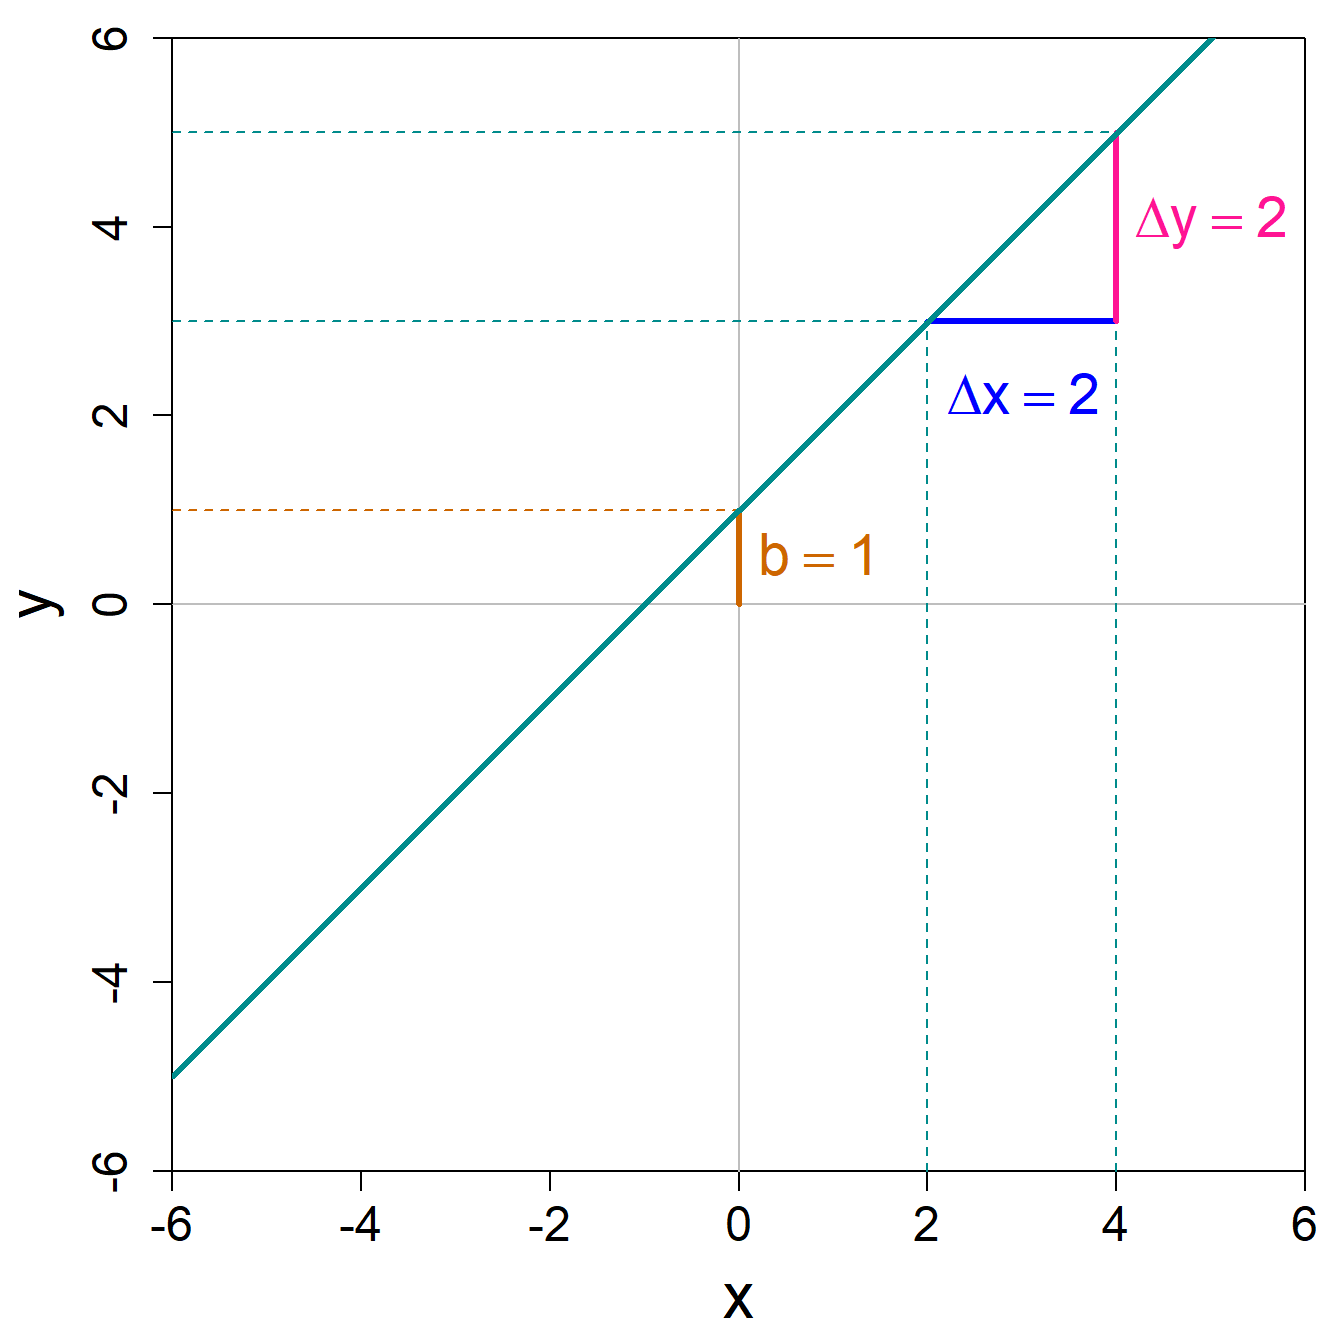
\includegraphics[width=0.5\linewidth]{02-basics_files/figure-latex/lin-func-1} 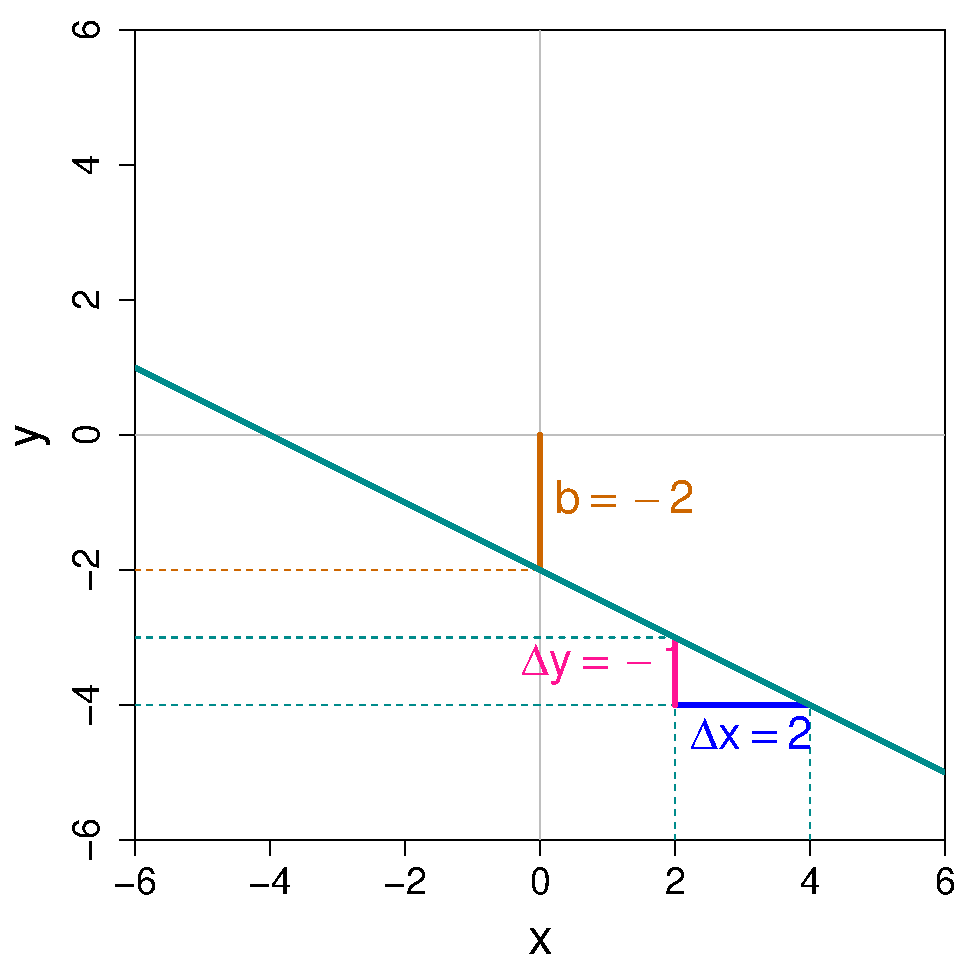
\includegraphics[width=0.5\linewidth]{02-basics_files/figure-latex/lin-func-2} 

}

\caption{Beispiele linearer Funktionen.}\label{fig:lin-func}
\end{figure}

Aus der linken Abbildung können wir ablesen, dass die Steigung dieser Geraden \(\frac{\Delta y}{\Delta x}=\frac{2}{2}=1\) ist und dass die Gerade die y-Achse am Ort \(1\) schneidet. Die entsprechende lineare Funktion kann dementsprechend als \(y = x + 1\) geschrieben werden.\footnote{Wir müssen hier die Steigung \(1\) nicht explizit schreiben, aber selbstverständlich ist es nicht falsch die lineare Funktion als \(y = 1\cdot x + 1\) zu schreiben.}

Aus der rechten Abbildung können wir ablesen, dass die Steigung \(\frac{\Delta y}{\Delta x}=\frac{-1}{2}=-0.5\) ist und dass die Gerade die y-Achse am Ort \(-2\) schneidet. Die entsprechende lineare Funktion kann dementsprechend als \(y = -0.5\cdot x -2\) geschrieben werden.

Es ist wichtig zu sehen, dass der Effekt einer Veränderung von \(x\) (also \(\Delta x\)) auf \(y\) überall derselbe ist. Es spielt also keine Rolle, ob wir von \(x=-2\) zu \(x=-1\) gehen oder von \(x=100\) zu \(x=101\), die entsprechende Veränderung in \(y\) (also \(\Delta y\)) wird dieselbe sein. Das muss so sein, denn die Gerade steigt (oder sinkt) mit konstanter Steigung.

\textbf{Aufgaben}

\begin{enumerate}
\def\labelenumi{\arabic{enumi}.}
\tightlist
\item
  Zeichnen Sie die Funktion \(y = 2\cdot x\) in ein Koordinatensystem ein. Warum fehlt der Parameter \(b\)?
\item
  Zeichnen Sie die Funktion \(y=-3\) in ein Koordinatensystem ein. Ist das überhaupt eine Funktion nach obiger Definition?
\end{enumerate}

\hypertarget{quadratische-funktionen}{%
\subsection{Quadratische Funktionen}\label{quadratische-funktionen}}

Nun wollen wir uns eine etwas interessantere (und flexiblere) Familie von Funktionen anschauen, nämlich \textbf{quadratische} Funktionen. Auch hier wollen wir die Funktion erstmal allgemein aufschreiben:

\[
y = f(x) = a \cdot x^2 + b \cdot x + c
\]
Eine quadratische Funktion hat drei \textbf{Parameter}, nämlich \(a\), \(b\) und \(c\). Grafisch entspricht die quadratische Funktion einer \textbf{Parabel} (vgl. Abb. \ref{fig:quad-func}). Die Parameter sind hier nicht mehr so einfach grafisch zu interpretieren, aber die vier Beispiele in unten stehender Abbildung geben Anhaltspunkte, was passiert, wenn die Parameterwerte sich ändern.

\begin{figure}

{\centering 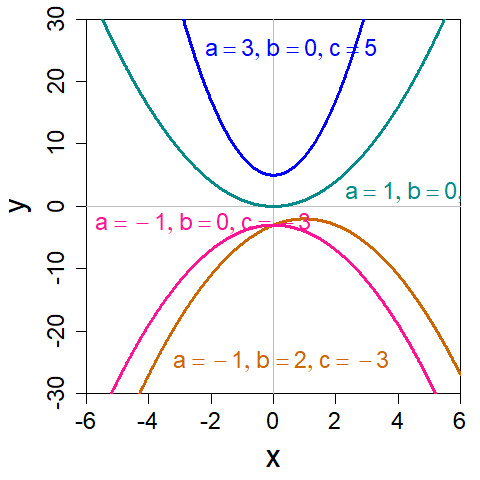
\includegraphics[width=0.8\linewidth]{02-basics_files/figure-latex/quad-func-1} 

}

\caption{Beispiele quadratischer Funktionen.}\label{fig:quad-func}
\end{figure}

\textbf{Aufgaben}

\begin{enumerate}
\def\labelenumi{\arabic{enumi}.}
\tightlist
\item
  Sie haben folgende quadratische Gleichung: \(y = 2 \cdot x^2 + x - 2\). Berechnen Sie mit der bekannten Lösungsformel \(x_{1,2}=\frac{-b \pm \sqrt{b^2 - 4ac}}{2a}\) die Orte auf der x-Achse, wo die Parabel die Achse schneidet (oder einfacher gesagt die Nullstellen).
\item
  Verwenden Sie folgenden R-Code, um beliebige quadratische Funktionen grafisch darzustellen, indem Sie die Parameterwerte auf der ersten Code-Zeile verändern.
\end{enumerate}

\begin{Shaded}
\begin{Highlighting}[]
\CommentTok{\# Parameter setzen}
\NormalTok{a }\OtherTok{\textless{}{-}} \DecValTok{2}\NormalTok{; b }\OtherTok{\textless{}{-}} \DecValTok{0}\NormalTok{; c }\OtherTok{\textless{}{-}} \DecValTok{1}
\CommentTok{\# Quadratische Funktion}
\NormalTok{quad }\OtherTok{\textless{}{-}} \ControlFlowTok{function}\NormalTok{(x, a, b, c) \{a }\SpecialCharTok{*}\NormalTok{ x}\SpecialCharTok{\^{}}\DecValTok{2} \SpecialCharTok{+}\NormalTok{ b }\SpecialCharTok{*}\NormalTok{ x }\SpecialCharTok{+}\NormalTok{ c\}}
\CommentTok{\# x{-}Werte}
\NormalTok{x }\OtherTok{\textless{}{-}} \FunctionTok{seq}\NormalTok{(}\SpecialCharTok{{-}}\DecValTok{6}\NormalTok{, }\DecValTok{6}\NormalTok{, }\FloatTok{0.01}\NormalTok{)}
\CommentTok{\# y{-}Werte}
\NormalTok{y }\OtherTok{\textless{}{-}} \FunctionTok{quad}\NormalTok{(x, a, b, c)}
\CommentTok{\# Plot}
\FunctionTok{plot}\NormalTok{(x, y, }\AttributeTok{type =} \StringTok{"l"}\NormalTok{, }\AttributeTok{lwd =} \DecValTok{2}\NormalTok{, }\AttributeTok{col =} \StringTok{"darkcyan"}\NormalTok{)}
\end{Highlighting}
\end{Shaded}

Sie wundern sich nun vielleicht, könnte man nicht auch eine Funktion antreffen, in der \(x^3\), \(x^4\), etc. vorkommen? Das ist selbstverständlich möglich. In diesem Fall spricht man dann von einem sogenannten \textbf{Polynom}. Die höchste Potenz des Arguments \(x\) definiert den Grad des Polynoms.

Schauen wir uns doch am besten gleich wieder ein Beispiel an:

\[
y = f(x) = 1 \cdot x^4 - 2 \cdot x^3 - 5 \cdot x^2 + 8 \cdot x - 2
\]
Die Visualisierung dieser Funktion ist in Abb. \ref{fig:poly-func} gegeben. Diese Funktion ist nun bereits enorm flexibel und kann je nach Parameterwerten ganz unterschiedliche Zusammenhänge abbilden.

\begin{figure}

{\centering 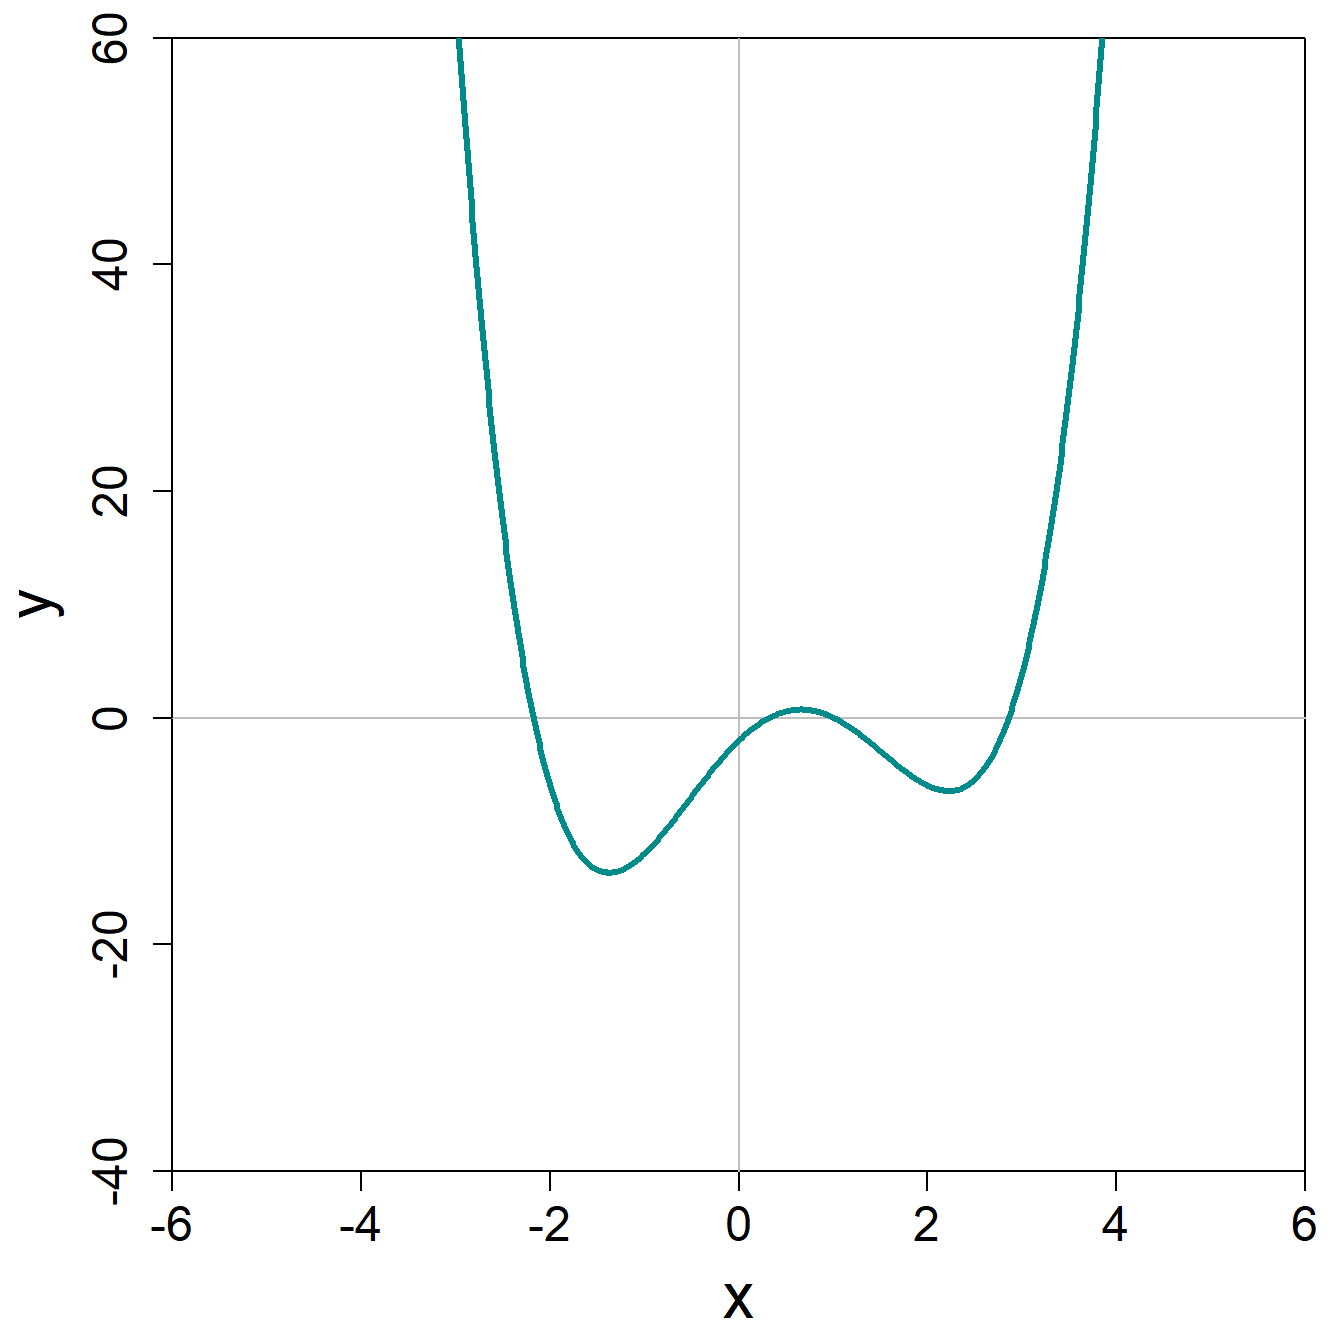
\includegraphics[width=0.8\linewidth]{02-basics_files/figure-latex/poly-func-1} 

}

\caption{Beispiel einer polynomischen Funktion vierten Grades.}\label{fig:poly-func}
\end{figure}

\textbf{Aufgaben}

\begin{enumerate}
\def\labelenumi{\arabic{enumi}.}
\tightlist
\item
  Eine quadratische Funktion ist ein Polynom welchen Grades?
\item
  Handelt es sich bei der Funktion \(y=2x^5 + x + 1\) immer noch um ein Polynom? Falls ja, ein Polynom welchen Grades?
\item
  Handelt es sich bei der Funktion \(y = x^{0.5} + 2\) um ein Polynom?
\end{enumerate}

\hypertarget{funktionen-mehrerer-argumente}{%
\subsection{Funktionen mehrerer Argumente}\label{funktionen-mehrerer-argumente}}

Bisher haben wir nur Funktionen mit \textbf{einem Argument} \(x\) angeschaut, doch die meisten für das Machine Learning interessanten Funktionen sind Funktionen \textbf{mehrerer Argumente}.

Der Einfachheit halber schauen wir uns hier nur mal eine \textbf{lineare} Funktion zweier Argumente, nennen wir sie \(x_1\) und \(x_2\), an, denn diese können wir in 3D immer noch visualisieren. Wir betrachten folgende Funktion: \(y = f(x_1,x_2) = 1 \cdot x_1 + 0.5 \cdot x_2 + 5\).

\begin{figure}

{\centering 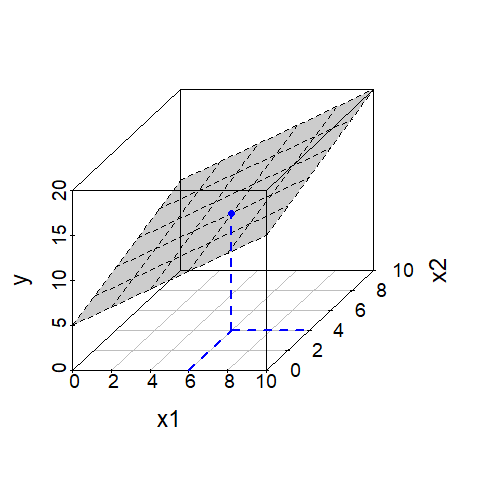
\includegraphics[width=0.8\linewidth]{02-basics_files/figure-latex/plane-1} 

}

\caption{Lineare Funktion zweier Argumente (Ebene).}\label{fig:plane}
\end{figure}

Aha! Während eine lineare Funktion eines Arguments grafisch einer Gerade entspricht, sehen wir nun, dass eine lineare Funktion zweier Argumente nichts anderes als eine Ebene darstellt. Wir sehen, dass die Ebene die y-Achse am Punkt \(5\) schneidet. Etwas schwieriger zu sehen ist die Steigung der Ebene in die Richtung der \(x_1\)-Achse und in die Richtung der \(x_2\)-Achse. Sie können aber vielleicht bereits erraten, dass die (partiellen) Steigungen \(1\) und \(0.5\) betragen.

Die Funktion ordnet jeden möglichen Punkt \((x_1,x_2)\) einem Punkt auf der Ebene zu. Wir können zum Beispiel für den in Abb. \ref{fig:plane} eingezeichneten Punkt \((6,4)\) den entsprechenden Punkt auf der Ebene ausrechnen:

\[ \begin{split}
y &= 1 \cdot x_1 + 0.5 \cdot x_2 + 5\\
&= 1 \cdot 6 + 0.5 \cdot 4 + 5\\
&= 13
\end{split}\]

Selbstverständlich könnten wir uns nun auch quadratische Funktionen oder Polynome mehrerer Argumente anschauen, aber darauf verzichten wir vorerst.

\hypertarget{potenzen-und-logarithmen}{%
\subsection{Potenzen und Logarithmen}\label{potenzen-und-logarithmen}}

Blabla\ldots{}

\hypertarget{integral--und-differentialrechnung}{%
\section{Integral- und Differentialrechnung}\label{integral--und-differentialrechnung}}

Olteanu materials:
Local vs.~global minima
From a maximization to a minimization problem
Basic definition of derivative
Differentiation rules
local min., max. and saddle point
Second derivative test
Partial derivatives
What is a gradient? What is Hessian? What is Jacobian?
Chain rules
Lagrange optimization

\hypertarget{lineare-algebra}{%
\section{Lineare Algebra}\label{lineare-algebra}}

Olteanu materials:
What is a scalar? What is a vector? What is a matrix?
Vector norms
Inner products
Symmetric, diagonal, square and identity matrix
Associative, commutative laws for matrices
Matrix addition and multiplication
Matrix inversion
Eigenvectors and eigenvalues
Quadratic form and positive (semi-) definiteness
Differentiation rules for matrices

\hypertarget{wahrscheinlichkeitsrechnung}{%
\section{Wahrscheinlichkeitsrechnung}\label{wahrscheinlichkeitsrechnung}}

Olteanu materials:
Sample space and axioms of probability
Conditional probability definition
Discrete vs.~continuous random variables
Joint probability distributions
Expectation and variance, covariance (always for discrete and continuous)
Bernoulli, Binomial, Normal, Multivariate Normal, Laplace

\hypertarget{diskrete-zufallsvariablen}{%
\subsection{Diskrete Zufallsvariablen}\label{diskrete-zufallsvariablen}}

Wir werden später sehen, dass im Machine Learning oftmals Dinge als \textbf{Zufallsvariablen} modelliert werden. Eine Zufallsvariable \(X\) ist eine Variable, für die der konkrete Wert nicht von vornherein klar ist. Wir können mit \(X\) zum Beispiel das Resultat eines Münzwurfs modellieren. Die zwei möglichen Resultate sind Kopf und Zahl. Vor dem Münzwurf ist nicht klar, ob Kopf oder Zahl erscheinen wird. Genau darum modellieren wir das Resultat des Münzwurfs als Zufallsvariable.

Es gibt in diesem einfachen Beispiel nur zwei mögliche Resultate (Kopf und Zahl), d.h. die Anzahl möglicher Resultate ist endlich (= nicht unendlich). Darum handelt es sich in diesem Fall um eine \textbf{diskrete} Zufallsvariable.

\hypertarget{verteilungen}{%
\section{Verteilungen}\label{verteilungen}}

\hypertarget{intro-R}{%
\chapter{Einführung in das Programmieren mit R}\label{intro-R}}

leaRn Materialen

tidymodels

Referenzen auf andere Ressourcen (Hadley et al.)

\hypertarget{lin-reg}{%
\chapter{Lineare Regression}\label{lin-reg}}

\hypertarget{lin-class}{%
\chapter{Lineare Klassifikation}\label{lin-class}}

\hypertarget{ml-pipeline}{%
\chapter{Machine Learning Pipeline}\label{ml-pipeline}}

\hypertarget{trees}{%
\chapter{Decision Trees}\label{trees}}

\hypertarget{ensembles}{%
\chapter{Ensembles}\label{ensembles}}

\hypertarget{svm}{%
\chapter{Support Vector Machines}\label{svm}}

\hypertarget{ann}{%
\chapter{Artificial Neural Networks}\label{ann}}

\hypertarget{cnn}{%
\chapter{Convolutional Neural Networks}\label{cnn}}

\hypertarget{rnn}{%
\chapter{Recurrent Neural Networks}\label{rnn}}

\hypertarget{gen-AI}{%
\chapter{Generative AI}\label{gen-AI}}

  \bibliography{book.bib,packages.bib}

\end{document}
